\section{Bipedal Locomotion Controller with I/O History}\label{sec:controller}
In this section, we describe the proposed general control framework for bipedal robots, leveraging the robot's dual I/O history as a fundamental element to enable transfer to environments with uncertain dynamics. 
This control architecture is the backbone of the RL system developed in this work, which will show advantages in terms of control performance in both the simulation and the real world. 

\paragraph{Control Framework}
Our locomotion control policy $\pi_\theta$ is represented by a deep neural network with parameters $\theta$. 
The same policy architecture will be used for a variety of different locomotion skills, and as such, it is crafted to rely on minimal skill-specific design choices. 
As shown in Fig.~\ref{fig:controller}, the policy outputs the desired robot motor positions $\mathbf{q}^d_{m}\in \mathbb{R}^{10}$ for the robot, which is the agent's action $\mathbf{a}_t$. 
The action is first smoothed by a Low Pass Filter~(LPF)~\citep{peng2020learning}, details of which are discussed in Appendix~\ref{appendix:lpf}. The filtered actions are then used by joint-level PD controllers to calculate the motor torques $\bm{\tau}$ that will be applied to the robot's actuated joints. The policy is queried at a rate of 33 Hz, whereas the PD controllers operate at a higher frequency of 2~kHz.


The policy's input at each timestep $t$ consists of four components: given command $\mathbf{c}_t$, reference motion $\mathbf{q}^r_t$, the robot's short I/O history $<\mathbf{o}_{t:t-4}, \mathbf{a}_{t-1:t-4}>$, and the robot's long I/O history $<\mathbf{o}_{t:t-65}, \mathbf{a}_{t-1:t-66}>$.
The time-varying command $\mathbf{c}_t$, as defined in Sec.~\ref{subsec:command} represents the task the robot is to accomplish using the desired locomotion skill. 
The locomotion skill is specified by a \emph{preview} of a skill-specific reference motion $\mathbf{q}^r_t$ at the current timestep $t$ for the robot.
It includes the incoming desired motor positions for the robot $\mathbf{q}^r_t=[\mathbf{q}^d_m(t+1), \mathbf{q}^d_m(t+4), \mathbf{q}^d_m(t+7)]$ which is sampled at timesteps that are 1, 4, and 7 ahead. 
The preview of the reference motion conveys the upcoming desired trajectory to the robot, aiding it in avoiding being shortsighted.
If the desired base height is not included in command $\mathbf{c}_t$, such as for running and jumping, the current base height from the reference motion $q^r_z(t)$ is then also included in the $\mathbf{q}^r_t$. 


\begin{figure}[t]
    \centering
    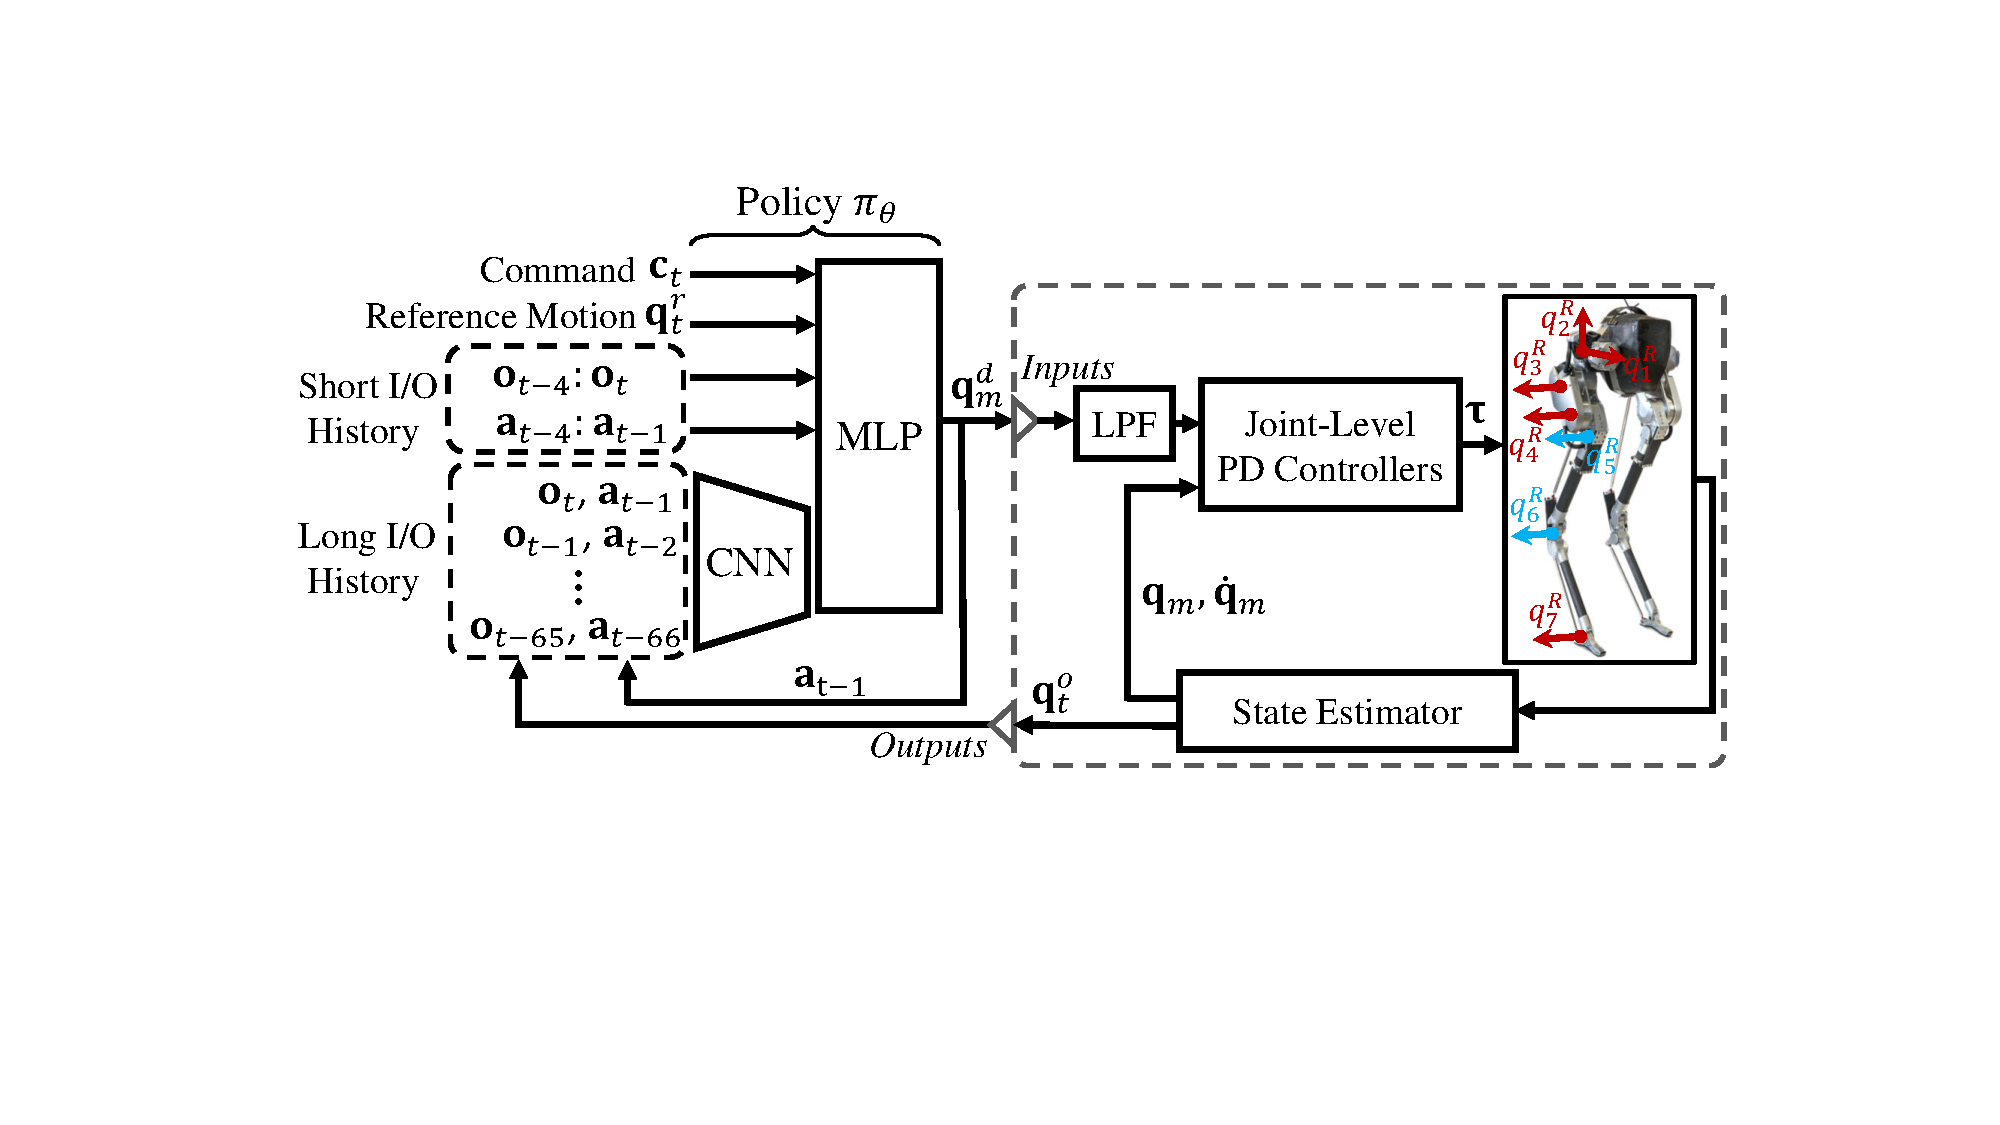
\includegraphics[width=\linewidth]{figures/controller.pdf}
    \caption{The proposed RL-based controller architecture that leverages a dual-history of input ($\mathbf{a}$) and output ($\mathbf{o}$) (I/O) from the robot. The control policy $\pi_\theta$, operating at 33 Hz, processes a 2-second long I/O history. This data is initially encoded via a 1D CNN along its time axis before being merged with a base MLP. In addition, a short history spanning 4 timesteps is directly input into the base MLP, combined with skill-specific reference motion $\mathbf{q}^r_t$ and variable commands $\mathbf{c}_t$ that parameterize the tasks. The policy outputs desired motor positions $\mathbf{q}^d_m$ as the robot's actions, which are then smoothed using a low-pass filter (LPF). These filtered outputs are employed by joint-level PD controllers operating at 2 kHz to specify motor torques $\bm{\tau}$. This architecture is general for various locomotion skills like standing, walking, running, and jumping. This figure also annotates the generalized coordinates for Cassie, which include actuated joints ($q^{L/R}_{1,2,3,4,7}$, marked as red) and passive joints ($q^{L/R}_{5,6}$, marked as blue).
    }
    \label{fig:controller}
\end{figure}



\paragraph{The use of Robot's I/O History} 
In addition to the observations described above, the observations also include a history of the robot's inputs and outputs (I/O) to the control policy. 
As depicted in Fig.~\ref{fig:controller}, the \emph{inputs} are represented by the desired motor positions (the robot's actions $\mathbf{a}$), while the \emph{outputs} are represented by the observable states of the robot, denoted as $\mathbf{o}$ and described in Sec.~\ref{subsec:states}.
This history is processed through two streams, which we refer to as a dual-history approach. 
The first stream offers a brief, four-timestep history of the robot's I/O, which is directly provided as input into the base network. 
This short history, lasting approximately 0.1 seconds, provides the robot with recent feedback for real-time control.
In addition to the short history, a longer I/O history, spanning two seconds, is also provided as input to the policy. This long history comprises of 66 pairs of robot I/O data ($<\mathbf{o}_{t-k}, \mathbf{a}_{t-k-1}>$, $k\in[0,65] \cap \mathbb{Z}$). 
This long I/O history contributes more to the identification of the system's dynamics, encompassing elements like the LPF, PD controllers, the robot itself governed by \eqref{eq:full_order_dynamics}, and its state estimator.
Such a structure allows the controller to effectively leverage information from both short-term and long-term I/O history. 
It is important to leverage both of these information. 
The long-term history is useful for system identification and inferring state estimates, especially for ballistic movements involved during the flight phase. 
The short-term history is also important from two perspectives: it can provide \emph{explicit} feedback of recent measurements on the robot, which is critical for real-time control, and it can help the robot to determine the weight of the past information which sometimes may not be important.
As we will show in Sec.~\ref{sec:policy_structure}, this dual-history structure leads to significant performance improvements for bipedal locomotion control. 



\paragraph{Details of Policy Representation}
As depicted in Fig.~\ref{fig:controller}, the policy architecture $\pi_\theta$ consists of two main components: a base network, modeled by a multilayer perceptron (MLP), and a long-term history encoder modeled by a 1D convolutional neural network (CNN), which computes an embedding of the long history that is provided as input to the base network.  
The base MLP has two hidden layers with 512 \textit{tanh} units each. 
The 1D CNN encoder consists of two hidden layers. 
Their configurations, defined as [kernel size, filter size, stride size], are [6, 32, 3] and [4, 16, 2] with \textit{relu} activation and no padding, respectively. 
The 66-timestep long I/O history is encoded via this CNN encoder through temporal convoluations along the time axis, and then compressed into a latent representation before being provided as input to the base MLP.
The output layer of the base MLP consists of \textit{tanh} units that specify the mean of the Gaussian distribution of the normalized action (w.r.t. the motor range). 
The standard deviation of the action distribution is specified by a fixed value $0.1I$.

\paragraph{General Policy Structure for Different Skills}
The control policy structure introduced in Fig.~\ref{fig:controller} is a general design and can be widely applied to a large variety of locomotion skills, such as standing, walking, running, and jumping. 
To train policies for different locomotion skills, a user needs only to simply provide different reference motions and commands to the policy, while the underlying architecture of the policy remains unchanged.
Throughout this paper, the same control policy architecture will be used for all experiments.
